\documentclass[conference]{IEEEtran}
\usepackage[utf8]{inputenc}
\usepackage{graphicx}
\usepackage[utf8]{inputenc}
\usepackage[T1]{fontenc}
\usepackage{graphicx}
\usepackage[space]{grffile}
\usepackage{longtable}
\usepackage{float}
\usepackage{wrapfig}
\usepackage{amssymb}
\usepackage{hyperref}
\usepackage{caption}
%\usepackage{epstojpg}
%\usepackage[jpg]{pstricks}
\usepackage{subcaption}
\usepackage{cite}
%\usepackage{subfigure}
\DeclareGraphicsExtensions{.eps}
%opening
\title{Large Scale Web Page Optimization of Virtual Labs}
%\author{Jatin Agarwal, Utkarsh Rastogi, Prateek Pandey, Maddala Saraswati Soumya and Venkatesh Chopella}

\begin{document}

\maketitle

\begin{abstract}
We propose web page optimization as a necessary step for virtual lab.
In context of virtual labs, several web applications were designed by people who are 
experts in their respective disciplines and hundreds of virtual labs were developed as a result.
Based on the complexity of each virtual lab, each lab developer decided to use his own 
set of tools and technologies, therefore virtual lab had lot of performance issues.
So end user suffered from slow rendering of pages on the client side.
Performance of a web application largely depends upon the content of the web
page because rendering takes place on client side. 
And client machine may have limited resources on his side. Therefore web page
optimization is a necessary step to improve user experience.
In contrast to existing work in this field, here we focus on large scale web
performance analysis through data visualization. This visualization gives a
us an understanding of performance issues of virtual labs. Based on this large scale visualization,
we present a utility of existing web optimization tools by experimentation of an
MHRD project virtual labs.
\end{abstract}

\section{Introduction}\label{sec-2}
Virtual Labs is a project initiated by the Ministry of Human Resource Development, Government of India,
under the National Mission on Education through Information and Communication Technology.
The project aims to provide remote-access to Laboratories in various disciplines of science
and engineering for students at all levels from under-graduate to research.
It also intends to develop a complete Learning Management System where the students can avail the
various tools for learning, including additional web-resources, video-lectures, animated demonstrations
and self-evaluation. There is also a component wherein costly equipment and resources are shared, which
are otherwise available to only a limited number of users due to constraints on time and geographical distances.
Seven IIT's (Delhi, Bombay, Kanpur, Kharagpur, Madras, Roorkee and Guwahati), IIIT Hyderabad, Amrita University,
Dayalbagh University, NIT Karnataka, and College of Engineering, Pune, are the institutions participating in the project.
The Project intends to cover physical sciences, chemical science and various branches of engineering like electronics and
communications, computer science and engineering, electrical engineering, mechanical engineering, chemical engineering,
biotechnology engineering and civil engineering.

After the onset of the world wide web, web performance implied optimizing the
server side but according to current trends
optimization on the client side has become bottle neck because of complex web
applications. 
{\it Critical rendering path} is the chain of necessary events that
occur to render web page on browser and resources fetched during critical rendering path are called 
{\it Critical Resources}\cite{crp}. Front-end developers use too many critical resources like
JavaScipt files, CSS files and images to make a good user interface which becomes
overhead during page rendering which means indigent user experience. Success of a web
application is judged based on user's experience which also depends upon fast response
time. Optimized web pages not only render fast but also save network
bandwidth. Along with a good responsive web page, web developers should
also focus on optimizing critical resources by minimizing size and number of resources.
For each critical resource on a web page, browser makes a new request to server.
CSS and javascript are the two critical resources that block the rendering of a web page.
Therefore, correct sequence of http requests can reduce the perceived page load time which means page
load time does not reduce in reality. So critical resources needed to render web page should be
fetched first and remaining resources should be fetched in the background. Therefore,
while optimizing web page for speed we should focus on \cite{crpo}
\begin{enumerate}
 \item Minimizing the size of critical resources
 \item Minimizing the number of critical resources
 \item Minimizing the critical rendering path.
\end{enumerate}

The goals of our experimentation, performed in collaboration with virtual labs were :

\begin{itemize}
\item To analyze performance of thousands of web pages hosted at virtual labs to improve students experience.
\item To evaluate the utility of {\it Pagespeed} in order to optimize web pages of virtual labs.
\item Comparison between the web performance of web pages of virtual labs with
and without a web optimization tool like {\it Google PageSpeed}.
\end{itemize}

\section{Background}\label{sec-3}
Initially when world wide web started most of the web pages where plain hyper text documents.
Slowly people started sharing media content like images and audio on web and in past decade
web pages got transformed into web application which depend upon on critical resources
like CSS, javascript and media content like images, audio, video etc. Now rendering of web pages depends upon
following three major criteria`s. Firstly order in which critical resources are fetched, secondly on
number of critical sources and lastly on size of critical resources. Web gaints like Yahoo and Google
have listed best practices for web developers to improve performance of web pages. So now we briefly
explain some of the best practices in order to appreciate the significance of web performance optimization,
for details explanation please refer to Yahoo's Best practices \cite{best-practices}.
\begin{itemize}
\item \textbf{Minimize http requests :}
Number of http requests to render any web page is directly proportional to
number of critical resources.
For each critical resource in the page, browser has to make a new http request 
to server and then it gets loaded. So, almost 80\% of the response time is
consumed in downloading all the resources. So to reduce number of http
requests, one can combine multiple CSS into one, also multiple javascript files can
be combined into one. Other ways include image spriting, etc.

\item \textbf{Use Content Delievery Networks :}
The nearest geographical server is selected for delivering the content which reduces network latency.

\item \textbf{Add Cache Control Header :}
For static components, setting far future {\it expires header} will reduce number of http request
so that browser can fetch resources from cache when request to same web page is made again.
For dynamic components, use an appropriate {\it Cache Control header} to help browser
with conditional requests. This reduces unnecessary http requests.

\item \textbf{Gzip components :}
Compression reduces response time by reducing the size of http response.
Gzip is most popular and effective compression method at this time. It reduces
response time by 70\%. If a web client indicates support for compression in
the {\it http request header} then server sends a compressed components.

\item \textbf{Stylesheets at the Top: }
Problem with not including link to style sheets in the head tag is that it blocks
progressive rendering and till the style sheets are not fetched users sees nothing
on screen.

\item \textbf{Put Scripts at Bottom :}
Putting scripts at the top, blocks parallel downloading of resources from same host.
In most of the cases scripts are needed when users start interacting with the web page and not during the rendering web page. 

\item \textbf{Make Inline Small CSS and javascript files :}
If file size is to small, then it should be made inline as it will reduce number
of the http requests.

\item \textbf{Make large css and javascript file external :}
CSS and javscript files are cached by browser. So we avoid downloading it every time a request is made.
First time it takes time to download but all later requests are served from the {\it browser cache}.

\item \textbf{ Minify javascript and css :}
Unnecessary characters from code should be reduced which includes removing
comments, redundant code and removing white spaces. Removing these unnecessary
characters reduces total number of critical bytes served to client-side and increases response time.

\item \textbf{Avoid Redirects :}
Connecting an old page to new one leads to an extra cycle of dns lookup and tcp handshake adding latency
and delaying the response. Therfore, it should be avoided.

\item \textbf{Configure ETags :}
Entity tags is a way that browser and server use to determine whether the
component in cache is same as that on server.

\item \textbf{Flush the buffer early :}
It allows to send partially ready response to browser. It should be written as
early as possible in the code, preferably in the head section.
In php there is a function flush() to flush the buffer. 

\item \textbf{No 404 error :}
Http requests are expensive and getting a response like '404 Not found' is totally useless
and adds to latency. Therefore, all such web pages should be avoided.

\item \textbf{Make favicon small and cacheable :}
Favicon stays in the core of server and  it is necessary because if its missing then
browser will still request for it and that adds to latency.
\end{itemize}

Yahoo {\bf Yslow}\cite{yslow} and {\bf Google Pagespeed}\cite{gps} are well known tools that are capable of
evaluating web pages' performance and providing suggestions to optimize web pages
based on the best practices listed above. But the pagespeed is more than a performance analysis
tool and is also capable of optimizing web pages without changing semantics of a web page.

Yahoo yslow.js is a javascript API which runs on phantomjs. PhantomJS is a
headless browser with JavaScript API\cite{pjs}. We used Yslow as performance measuring
tool because it not only analyzes a web page but gives suggestions on how to
improve it. It works on following three ways:
\begin{itemize}
\item It crawls the DOM to find each component.
\item Collects information from each component and analyzes each of them.
\item It generates scores out of 100 for each rule which produces the overall
score for page.
\end{itemize}
The grades for individual rules are computed differently depending on the rule.
For example, for Rule 1, three external scripts are allowed and each extra script
four points are deducted from the overall weight. The code for grading each
rule is found in rules.js. The overall grade is a weighted average of the
individual grades for each rule, calculated in controller.js. The rules are applied
approximately in order of importance, most important first. The specific weights
are in the ruleset objects in rules.js. For details on score computation please refer to Rule Matrix\cite{rulematrix}.

Mod\_pagespeed\cite{google:mod-pagespeed} is an automated web page optimization tool developed by Google for
optimization of web pages. It not only
analyzes a web page but also optimizes it. Based on best practices, it has
certain set of filters which optimizes web page during run time. As the server
gets request for the web page, it dynamically rewrites the page using its filters\cite{pagespeed:filters}
and sends a highly optimized page. The rewriting happens only when the first
request for web page is made and for all later requests web page is served from the cache
at server side. There are more than 40 filters which support
optimization. These filters can be turned on or off based on requirements. 
% 
% 
\section{Approach}\label{sec-4}
Our work is broadly divided into four major phases namely Data Collection, Data
Visualization, Analysis of Data and optimizing web pages based on analysis.
During data collection phase we first collected all the urls of virtual labs
hosted on www.deploy.virtual-labs.ac.in. Then we collected {\it Yslow} reports for each web page
using an automated script and phantomJs. After collecting all the reports we
extracted scores for each rule from reports and stored it in a csv file. During
visualization phase all data is visualized using an automated script indicating
performance for each rule and also overall performance of web pages. Later we
carried out analysis to optimize the web pages of virtual labs.

\subsection{Urls and Report Collection}\label{sec-4.1}
As a first step to collect data and generate reports, we
collected urls of all the web pages at following domain deploy.virtuals-labs.ac.in.
Since we have access to server, to get all the urls, we extracted
all the html and php pages' links from the server and stored it into the text file
using an automated bash script.
In order to test the performance of web pages www.vlab.co.in, we collected the 5000 urls
using an online sitemap generator since we did not had access to server.
We extracted {\it yslow} report for each web page using yslow.js and phantomJS using automated bash
script. This automated script read the url line by line from a text file containing
urls and generated a report for each web page. This script does batch processing running
ten phantomjs processes in background for ten different web pages. The urls of dangling web pages 
are pushed into a text file named failed-urls and such reports are deleted.
These {\it ylsow} reports serves as input to CSV file generation.

\subsection{CSV File Generation}\label{sec-4.2}
CSV file are generated using a bash script. This CSV file contains the overall
score and scores corresponding to each rule. Script extracts all the scores
corresponding to each rule and dumps it into the CSV file line by line. The
content in the CSV file is used for visualizing statistics.

\subsection{Data Visualization}\label{sec-4.3}
Data visualization is carried out using python matplotlib \cite{matplot} and csvkit \cite{csvkit}. 
Statistics for each rule is plotted using an automated
script in the form of bar graphs as shown in Appendix \ref{appendixx}. Scripts take csv files as input
and return set of bar graphs specific to each rule as output.

\section{Experimentation}\label{sec-5}
In order to achieve our goals we carried out experimentation on three different set of urls:
\begin{enumerate}
 \item set containing 4945 urls of {\it www.vlab.co.in} without {\it pagespeed}
 \item set containing 8786 urls of {\it www.deploy.virtual-labs.ac.in} without {\it pagespeed}
 \item set containing 8786 urls of {\it www.deploy.virtual-labs.ac.in} with pagespeed
\end{enumerate}
For each of the above set of urls we generate {\it yslow} reports and accumulate scores
in three different CSV files. Later statistics are visualized in the form of bar graphs for each csv file.
We analyze the performance of www.vlab.co.in using obtained bar graphs in next section.
We also studied comparison between performance of 8786 web pages of www.deploy.virtual-labs.ac.in
with and without {\it pagespeed}.

% \subsection{Analysis of performance for 5000 web pages of www.vlab.co.in}\label{sec-5.1}
% We started our experiment by collecting {\it yslow} reports for vlabs. 
% We collected 5000 urls of www.vlab.co.in. and generated
% {\it Yslow} reports of the corresponding web pages and generated a CSV file for the
% scores. Finally, we plotted data accumulated in the csv file and analyzed the
% current status of web pages by looking at bar graphs.
% 
% \subsection{Data collection for deploy.virtual-labs.ac.in without pagespeed}\label{sec-5.2}
% In order to analyze performance of web pages, we collected all the urls located at deploy.virtual-labs.ac.in byCritical using
% our bash script. Total of 8786 urls were collected, reports were
% generated for each web page located at respective url and scores were accumulated in a csv file.
% Later statistics are visualized to analyze the performance.
% 
% \subsection{Data collection for deploy.virtual-labs.ac.in with pagespeed}\label{sec-5.3}
% The replica of deploy.virtual-labs.ac.in server is made on a container and
% Google {\it mod\_pagespeed} was installed on it.
% Then reports were collected for all the 8786 web pages and a CSV file was generated.
% The obtained statistics were compared with results of deploy.virtual-labs.ac.in without pagespeed
% to observe how much optimization was done by pagespeed.
\section{Analysis}\label{sec-6}
In this section we analyze web page performance of {\it www.virtual-labs.ac.in} in two different settings on a data set containing 8786 web pages.
One when page speed module is installed on our system, other one without it. We also analyze web page performance of vlab.co.in  
on data set containing 4945 web pages.
\subsection{Analysis of performance for 5000 web pages of {\it www.vlab.co.in}}
 Out of 5000 urls, we collected statistics for 4945 web pages. Note that all figures are placed in the Appendix Section.
\begin{itemize}
\item From the bar graph in figure \ref{overallscore-vlab}, we can observe that only 1 web page is having good
performance. Rest of the web pages do not get good grades and need to be
optimized to improve performance. Out of rest 687 i.e 13\% of the web pages are in above average conditions, 1038
web pages are performing average and rest 3220 web pages are not in good
condition. Therefore, these statistics show that these pages are not following
best practices and performance of web pages can be improved.  
 
\item From the bar graph in figure \ref{fig:cssattop}, we can observe that all the web pages are having their
CSS files inside the head tag else they would block the progressive rendering.

\item From the bar graph in figure \ref{fig:jsatbottom}, we can observe that all the web pages are having their
script files at the bottom else they would block the parallel downloading.

\item From the bar graph in figure \ref{fig:usecdn}, we can observe there is no usage of Content Delivery
Networks(CDN). It is suggested to use CDN's for large web sites like www.vlab.co.in in order to reduce latency.

\item From the bar graph in figure \ref{fig:add-eh}, we can observe that there is no use of {\it Expires
Headers} in the web pages. If this practice is not followed in the web pages then it has to
fetch each static critical resource every time page is requested.

\item From the bar graph in figure \ref{fig:ccg}, we can observe that only 89 web pages out of 4945
pages are in compressed form and rest are in uncompressed form. This will lead to
large payload size and will increase network traffic and will slow page rendering.

\item From the bar graph in figure \ref{fig:configure-et}, we can observe that this website does not use entity
tags. Due to this it has to download critical resources every time request for page is made.

\item From the graph in figure \ref{fig:favicon}, we can see that all web pages of vlabs are having favicon for it.

\item From the graph in figure \ref{fig:httpr}, we can see that number of critical resources on the pages
are more than required. Only 1 web page is getting A+ grade. Around 4500 web pages
have scores between 65 to 75 meaning that they are loaded with multiple css, javascript
and images. For each resource, browser has to make a request to server and most
of the time it is wasted downloading the resources. Number of resources should be
reduced for fast rendering.
\end{itemize}

\subsection{Comparison with and without {\it Pagespeed}}\label{sec-6.2}
We have generated statistics for 8786 web pages under
deploy.virtual-labs.ac.in without {\it pagespeed} and for replica of deploy server with {\it pagespeed}
installed. Here we observed how much {\it pagespeed} optimizes the web pages in comparison
when pagespeed is not used. Note that all figures are placed in the Appendix Section.
\begin{itemize}
\item From the bar graph in figure \ref{fig:overallscore-comparison} we can notice that 4299 web pages fall under
A+ grade for \textbf{overall score} while with pagespeed this rises to 6051. It
shows pagespeed is improving the performance of web pages by about 20\%. Also
we can see that without pagespeed only 1226 web pages are in A- grade but with
pagespeed it increased to 1667. From the figure \ref{fig:overallscore-comparison} we can observe that overall
performance of web pages has improved after using pagespeed.

\item From the bar graphs in figure \ref{fig:addexpireheader-comparison}, we can observe that without pagespeed only 3214
web pages are in B+  use \textbf{added expires headers} and around
45\% are not using it. But with pagespeed, 4729 web pages were in B+ grade and
there was shift of number from low grades to high grades.

\item From the bar graphs in figure \ref{fig:ccg-comparison}, we can observe that most web pages follow \textbf{compressed
using Gzip} rule and 8257 urls falls under A+ grades while with pagespeed this number rises to 8761.

\item From the bar graphs in figure \ref{fig:etag-comparison},
we can observe that \textbf{Etags rule} without pagespeed
3535 pages have A+ grade, 831 have B+ grade, 384 have C+ grade, 3704 have score
below than 50 but with pagespeed this number shifted to more higher grades. We can
see now 6441 pages fall in  A+ compared with 3534 pages without pagespeed. But the major difference is seen
at below 50 score pages, now this have reduced to 633 in comparison to previous
3704.

\item From the bar graphs in figure \ref{fig:httpr-comparison}, we can see that w.r.t \textbf{make fewer http
requests} rule, without pagespeed only 7791 web pages were in grade A+ and 461 pages
were in A- but with pagespeed 8202 pages were in A+ grades. Major shift was from 
A- grade to A+ grade. Rest pages shows no observable changes.

\item From the bar graphs in figure \ref{fig:minify-comparison}, we can see that \textbf{minified JavaScript and CSS} rule
without pagespeed 7059 web pages were in grade A+, 1395 pages in A-, then 254 in
B- and 20 were below F. After optimizing with pagespeed 8639 pages were in grade A+ ,94 in A- and only 3 below F.
\end{itemize}

\section{Conclusion and Future Work}
\label{sec-7}
This paper is concerned about Web Page Optimization of virtual labs in order to improve user experience.
This optimization is achieved by minimizing the number of critical resources, minimizing the size of
critical resources and minimizing the critical path length. Our framework helped us in visualizing web performance and
provide suggestions to developers to improve performance. It also gives the list of urls of dangling web pages.
Our comparison study asserts that Google Pagespeed as strong utility for optimizing web applications.
It should be used for huge websites like virtual labs, where various domains and backgrounds are involved.
 
%\section{Future Work}\label{sec-8}
This framework can be modified to give the list of urls of web pages that perform badly.
Generating report takes at least 24 hrs to process 5000 urls but by
making phantomjs clusters on framework like Hadoop we can parallelize the whole report generation.
Also, the functionality of pagespeed can be improved by developing more filters. For example, there is no filter to give default
favicon for a web page.

\begin{thebibliography}{1}
\bibitem{crp}
Google Developers. Analyzing The Critical Rendering Path\\
\href{
https://developers.google.com/web/fundamentals/performance/critical-rendering-path/analyzing-crp}
{https://developers.google.com/web/fundamentals/performance/critical-rendering-path/analyzing-crp}

\bibitem{crpo}
Google Developers. Optimizing The Critical Rendering Path:\\
\href{
https://developers.google.com/web/fundamentals/performance/critical-rendering-path/optimizing-critical-rendering-path}
{https://developers.google.com/web/fundamentals/performance/critical-rendering-path/optimizing-critical-rendering-path}

\bibitem{best-practices}
Yahoo Developer Network--Best Practices for Speeding Up Your Website:\\
\href{https://developer.yahoo.com/performance/rules.html}{
https://developer.yahoo.com/performance/rules.html}

\bibitem{yslow}
Yslow Official Website.Available:\\
\href{http://yslow.org/phantomjs/}{http://yslow.org/phantomjs/
}

\bibitem{gps}
Google Pagespeed Tools.Official Documentation:\\
\href{https://developers.google.com/speed/pagespeed/}{
https://developers.google.com/speed/pagespeed/}

\bibitem{pjs}
PhantomJs:\\
\href{http://phantomjs.org/}
{http://phantomjs.org/}

\bibitem{rulematrix}
Yslow Score Computation:\\
\href{http://yslow.org/ruleset-matrix/}
{http://yslow.org/ruleset-matrix/}

\bibitem{google:mod-pagespeed}
Google Mod\_pagespeed.Available:\\
\href{
https://developers.google.com/speed/pagespeed/module}{
https://developers.google.com/speed/pagespeed/module}
 
\bibitem{pagespeed:filters}  
Pagespeed Filters:\\
\href{https://developers.google.com/speed/pagespeed/module/filters}
{https://developers.google.com/speed/pagespeed/module/filters}

\bibitem{matplot}
Matplotlib:\\
\href{http://matplotlib.org/}
{http://matplotlib.org/}

\bibitem{csvkit}
CSV Kit:\\
\href{https://csvkit.readthedocs.org/en/0.8.0/}
{https://csvkit.readthedocs.org/en/0.8.0/}
% 
% \bibitem{wpo08}
% Andrew B.King, 2008. Website Optimization : Web performance
% Optimization. 155-185,282-290.
% 
% \bibitem{ss07}
% Steve Souders, 2007.  High Performance Websites. 10-84
% 
% \bibitem{ss09}
% Steve Souders, 2009. Even Faster Web Sites

\end{thebibliography}
%\newpage
\appendix
\label{appendixx}
%\section{Comparison before optimization and after optimization using for deploy.virtual-labs.ac.in}
%\section{figures}
\begin{figure}[ht]
  \centering
  $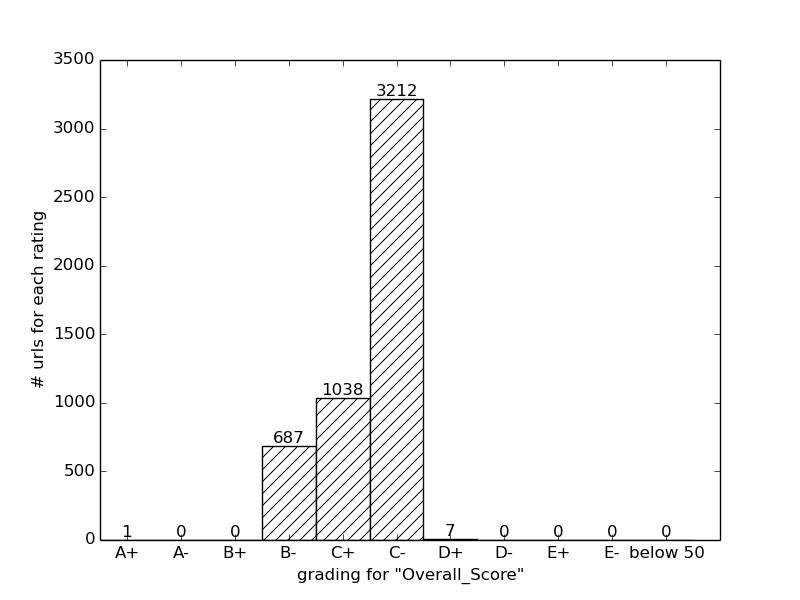
\includegraphics[scale=0.33]{new-img-jpg/vlab-jpg/Overall_Score.jpg}$
  \caption{Number of urls versus Overscore}
  \label{overallscore-vlab}
\end{figure}

\begin{figure}[ht]
 \centering
  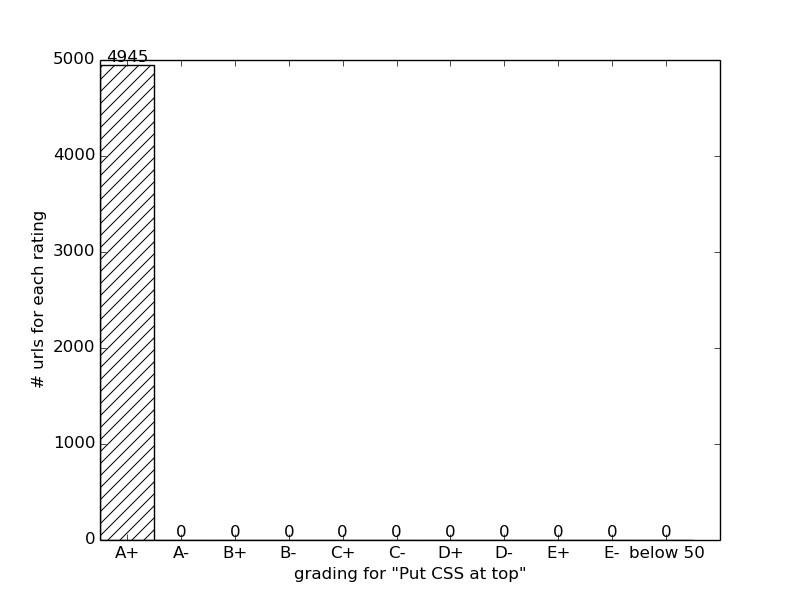
\includegraphics[scale=0.33]{new-img-jpg/vlab-jpg/Put CSS at top.jpg}
\caption{Number of urls versus Put CSS at top}
\label{fig:cssattop}
\end{figure}

\begin{figure}[ht]
 \centering
  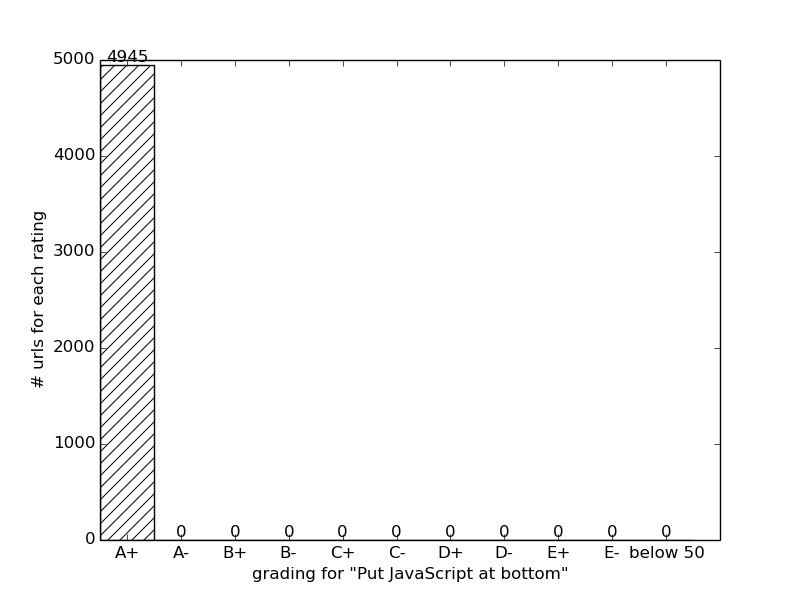
\includegraphics[scale=0.33]{img/vlab+/Put JavaScript at bottom.jpg}
\caption{Number of urls versus Put JavaScript at bottom}	
\label{fig:jsatbottom}
\end{figure}
           
\begin{figure}[ht]
 \centering
  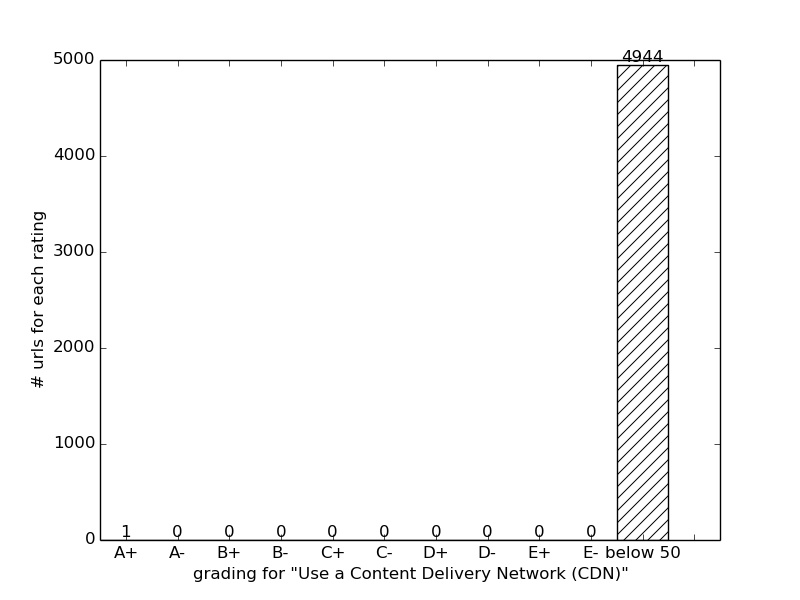
\includegraphics[scale=0.33]{new-img-jpg/vlab-jpg/Use a Content Delivery Network (CDN).jpg}
\caption{Number of urls versus Use a Content Delivery Network (CDN)}	
\label{fig:usecdn}
\end{figure}        

\begin{figure}[ht]
 \centering
  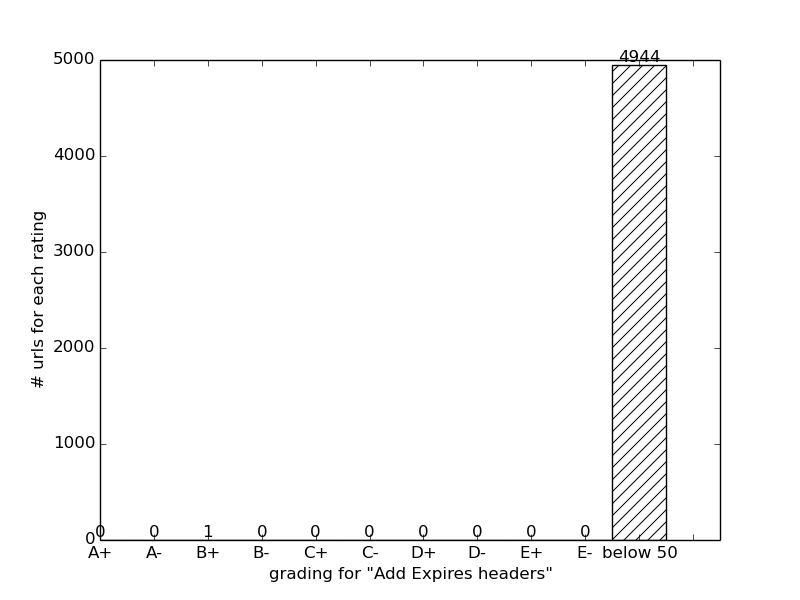
\includegraphics[scale=0.33]{new-img-jpg/vlab-jpg/Add Expires headers.jpg}
\caption{Number of urls versus Add Expires Headers}	
\label{fig:add-eh}
\end{figure}

\begin{figure}[ht]
 \centering
  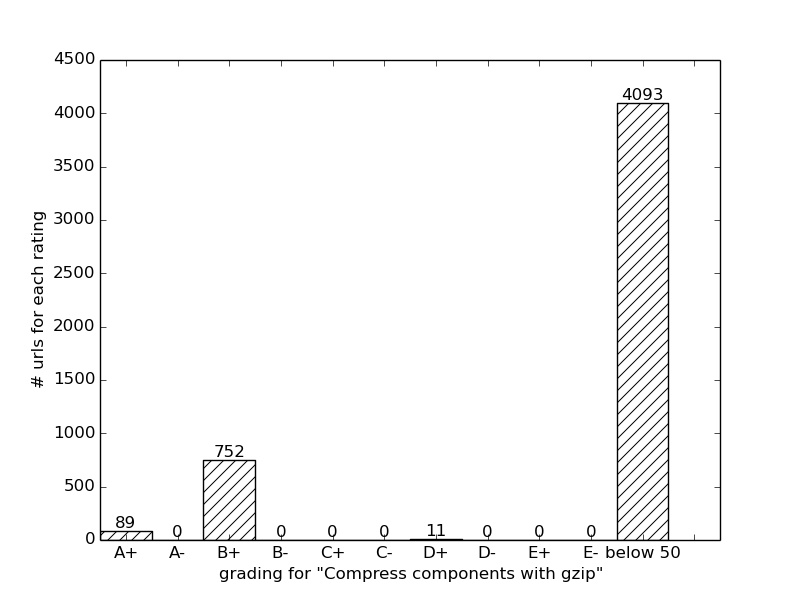
\includegraphics[scale=0.33]{new-img-jpg/vlab-jpg/Compress components with gzip.jpg}
\caption{Number of urls versus Compress components with gzip}	
\label{fig:ccg}
\end{figure}

\begin{figure}[ht]
 \centering
  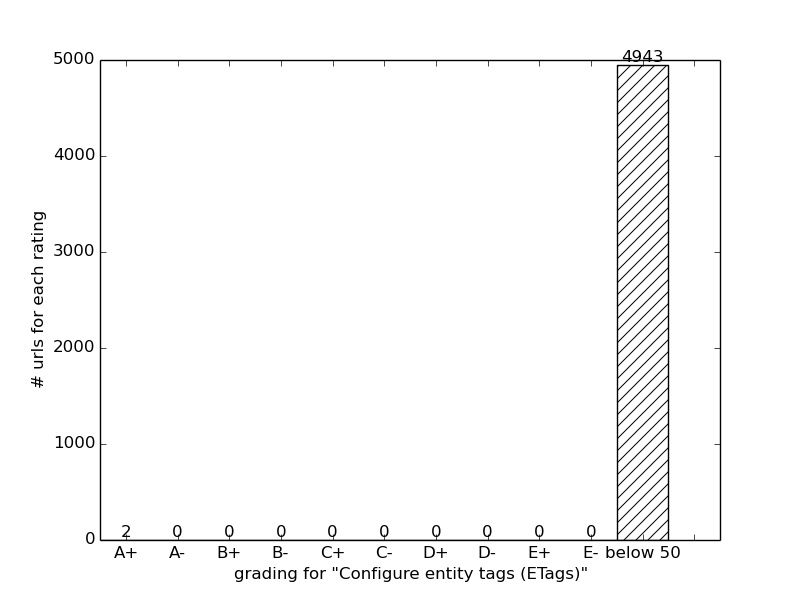
\includegraphics[scale=0.33]{new-img-jpg/vlab-jpg/Configure entity tags (ETags).jpg}
\caption{Number of urls versus Configure entity tags (ETags)}	
\label{fig:configure-et}
\end{figure}

\begin{figure}[ht]
 \centering
  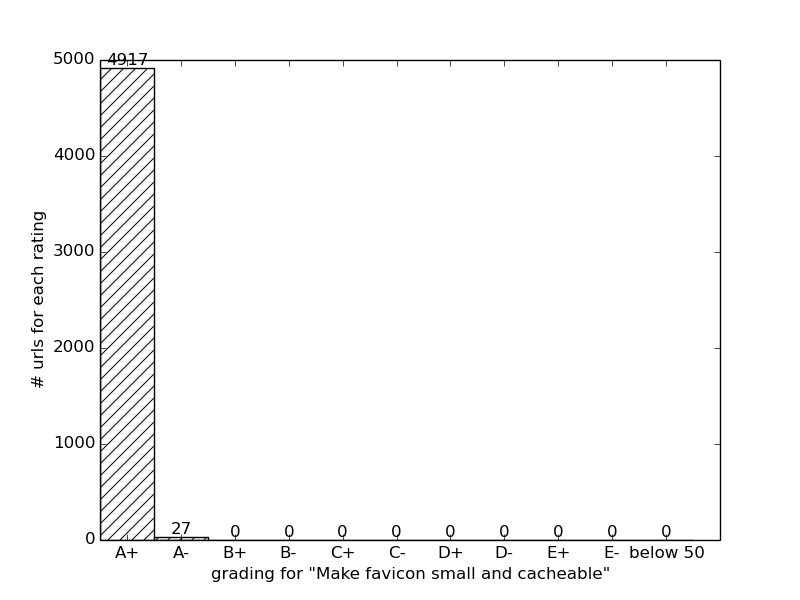
\includegraphics[scale=0.33]{new-img-jpg/vlab-jpg/Make favicon small and cacheable.jpg}
\caption{Number of urls versus Make favicon small and cacheable}	
\label{fig:favicon}
\end{figure}

\begin{figure}[ht]
 \centering
  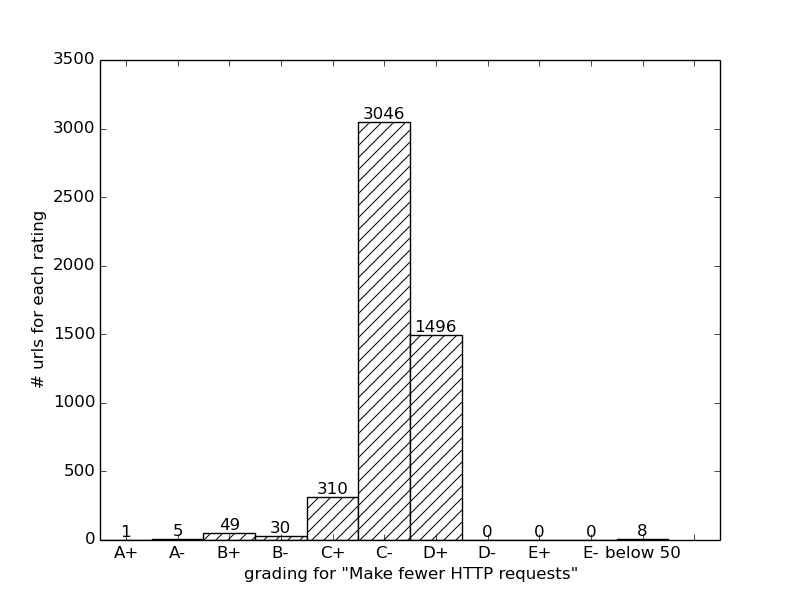
\includegraphics[scale=0.33]{new-img-jpg/vlab-jpg/Make fewer HTTP requests.jpg}
\caption{Make fewer HTTP requests Versus Number of urls}	
\label{fig:httpr}
\end{figure}

\begin{figure*}
    \centering
    \begin{subfigure}[b]{\columnwidth}        %% or \columnwidth
        \centering
	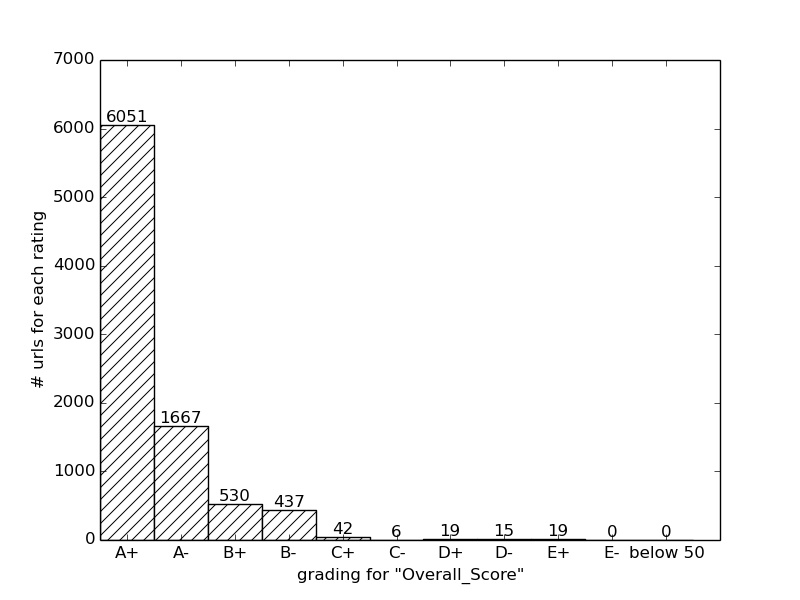
\includegraphics[scale=0.33]{new-img-jpg/container-jpg/Overall_Score.jpg}
        \caption{Overall Score With PageSpeed}
        \label{fig:overallscore-pagespeed}
    \end{subfigure}
    \hfill
    \begin{subfigure}[b]{\columnwidth}        %% or \columnwidth
        \centering
	 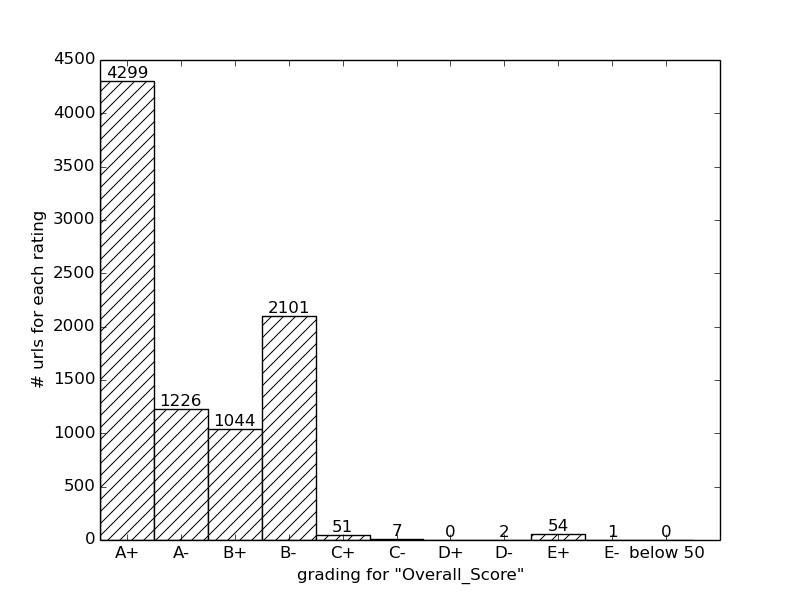
\includegraphics[scale=0.33]{new-img-jpg/deploy-jpg/Overall_Score.jpg}
        \caption{Overall Score without PageSpeed}
        \label{fig:overallscore-nopagespeed}
    \end{subfigure}
    \caption{Comparing Overall Scores}
    \label{fig:overallscore-comparison}
\end{figure*}

\begin{figure*}
    \centering
    \begin{subfigure}[b]{\columnwidth}        %% or \columnwidth
        \centering
	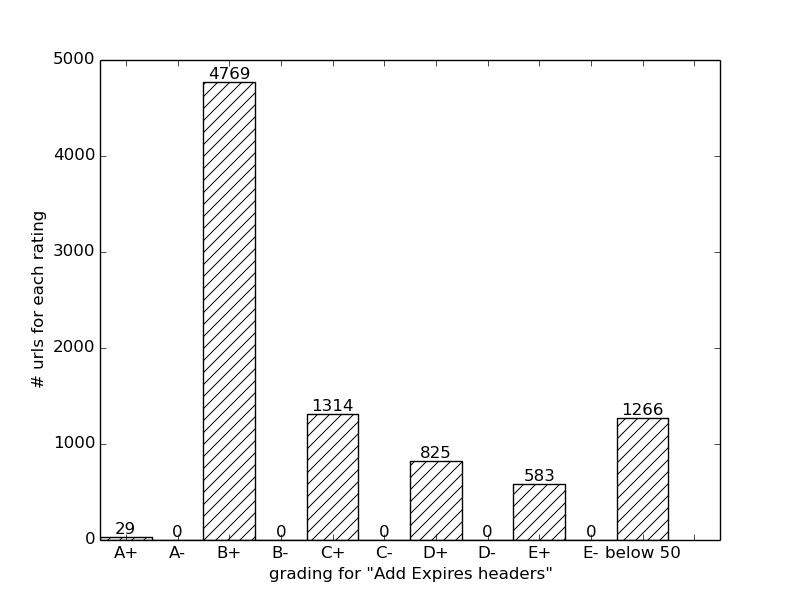
\includegraphics[scale=0.33]{new-img-jpg/container-jpg/Add Expires headers.jpg}
        \caption{'Add Expires Header' Rule with PageSpeed}
        \label{fig:addexpireheader-pagespeed}
    \end{subfigure}
    \hfill
    \begin{subfigure}[b]{\columnwidth}        %% or \columnwidth
        \centering
  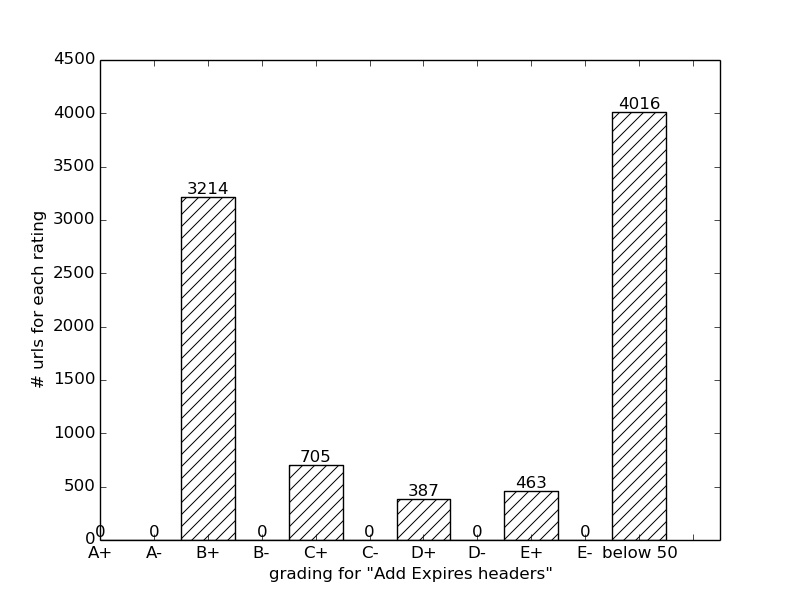
\includegraphics[scale=0.33]{new-img-jpg/deploy-jpg/Add Expires headers.jpg}
        \caption{'Add Expires Header' Rule without PageSpeed}
        \label{fig:addexpireheader-nppagespeed}
    \end{subfigure}
    \caption{Comparing 'Add Expire Header' rule}
    \label{fig:addexpireheader-comparison}
\end{figure*}

\begin{figure*}
    \centering
    \begin{subfigure}[b]{\columnwidth}        %% or \columnwidth
        \centering
	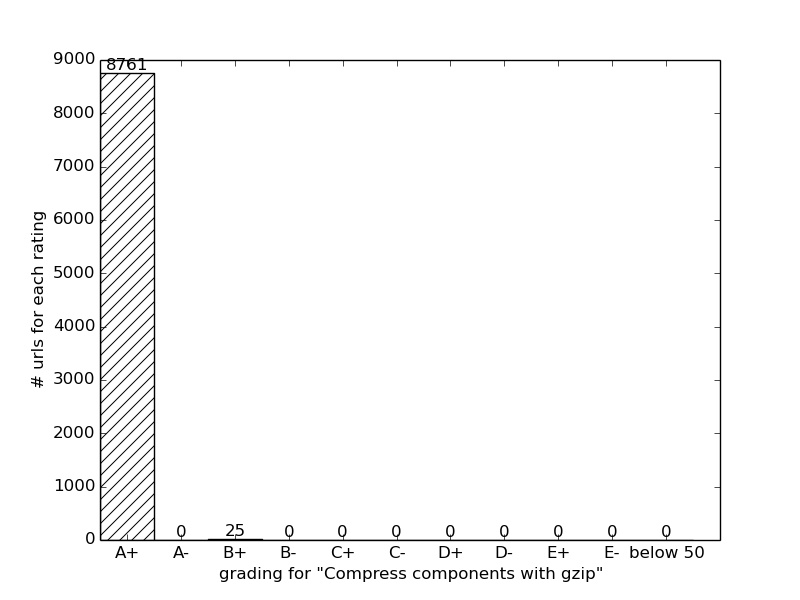
\includegraphics[scale=0.33]{new-img-jpg/container-jpg/Compress components with gzip.jpg}
        \caption{'Compress Components with gzip' rule with PageSpeed}
        \label{fig:ccg-pagespeed}
    \end{subfigure}
    \hfill
    \begin{subfigure}[b]{\columnwidth}        %% or \columnwidth
        \centering
	 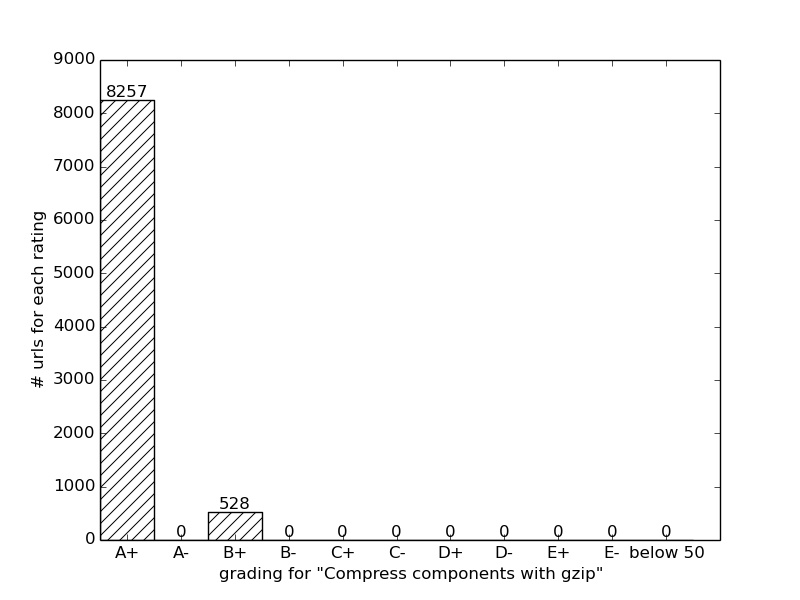
\includegraphics[scale=0.33]{new-img-jpg/deploy-jpg/Compress components with gzip.jpg}
        \caption{'Compress Components with gzip' rule without PageSpeed}
        \label{fig:ccg-nopagespeed}
    \end{subfigure}
    \caption{Comparing 'Compress Components with gzip' rule}
    \label{fig:ccg-comparison}
\end{figure*}

\begin{figure*}
    \centering
    \begin{subfigure}[b]{\columnwidth}        %% or \columnwidth
        \centering
	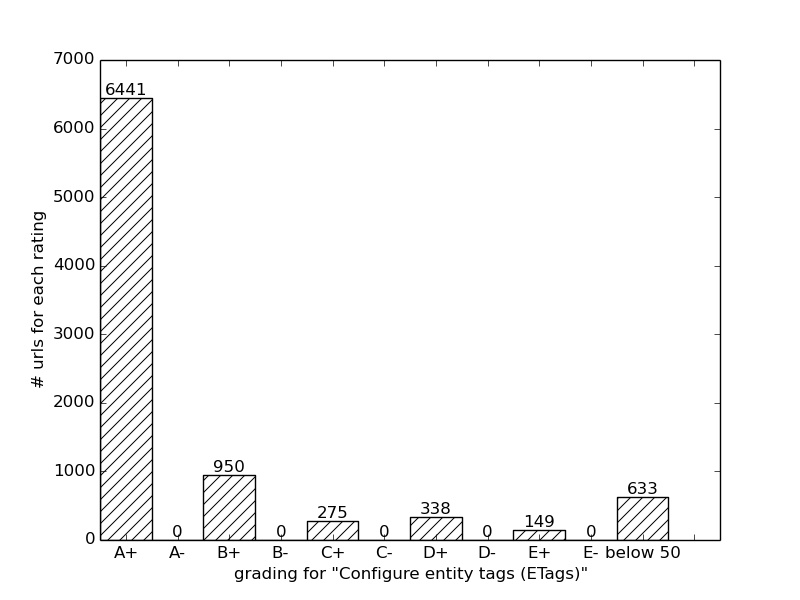
\includegraphics[scale=0.33]{new-img-jpg/container-jpg/Configure entity tags (ETags).jpg}
        \caption{'Configure entity tags (ETags)' rule with PageSpeed}
        \label{fig:etag-pagespeed}
    \end{subfigure}
    \hfill
    \begin{subfigure}[b]{\columnwidth}        %% or \columnwidth
        \centering
	 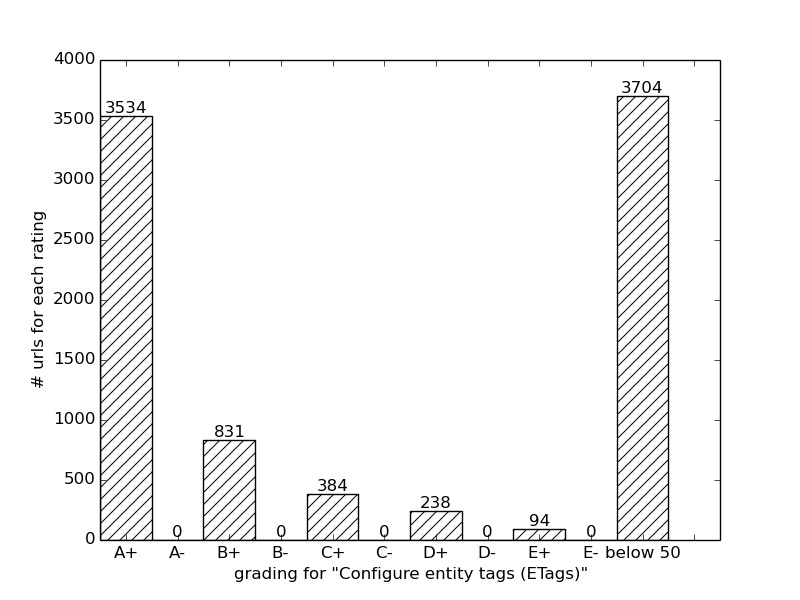
\includegraphics[scale=0.33]{new-img-jpg/deploy-jpg/Configure entity tags (ETags).jpg}
        \caption{'Configure entity tags (ETags)' rule without PageSpeed}
        \label{fig:etag-nopagespeed}
    \end{subfigure}
    \caption{Comparing 'Configure entity tags (ETags)' rule}
    \label{fig:etag-comparison}
\end{figure*}

\begin{figure*}
    \centering
    \begin{subfigure}[b]{\columnwidth}        %% or \columnwidth
        \centering
	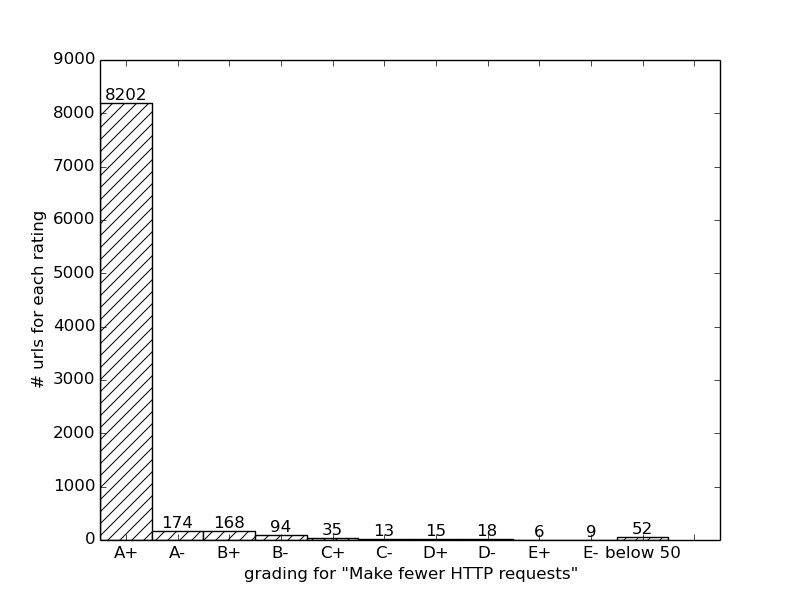
\includegraphics[scale=0.33]{new-img-jpg/container-jpg/Make fewer HTTP requests.jpg}
        \caption{'Make fewer HTTP requests' rule with PageSpeed}
        \label{fig:httpr-pagespeed}
    \end{subfigure}
    \hfill
    \begin{subfigure}[b]{\columnwidth}        %% or \columnwidth
        \centering
	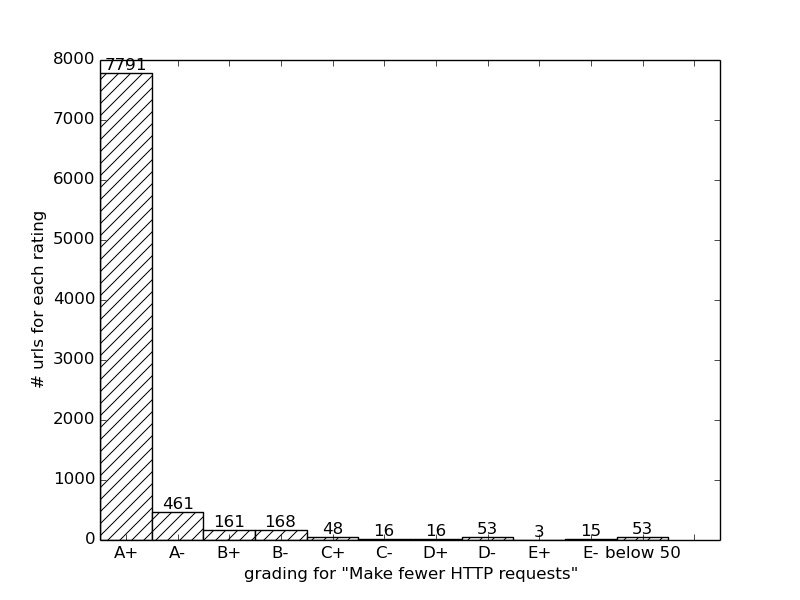
\includegraphics[scale=0.33]{new-img-jpg/deploy-jpg/Make fewer HTTP requests.jpg}
        \caption{'Make fewer HTTP requests' rule with PageSpeed}
        \label{fig:httpr-nopagespeed}
    \end{subfigure}
    \caption{Comparing ''Make fewer HTTP requests' rule}
    \label{fig:httpr-comparison}
\end{figure*}

\begin{figure*}
    \centering
    \begin{subfigure}[b]{\columnwidth}        %% or \columnwidth
        \centering
        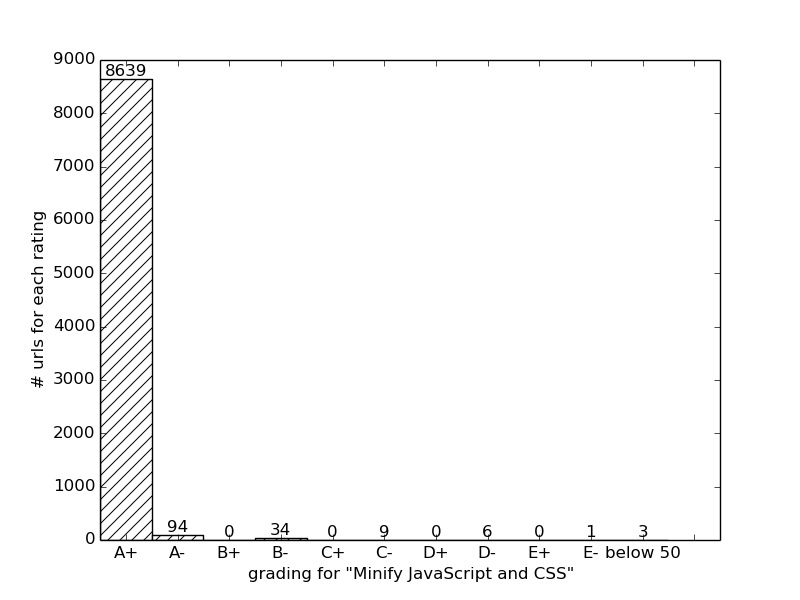
\includegraphics[scale=0.33]{new-img-jpg/container-jpg/Minify JavaScript and CSS.jpg}
        \caption{'Minify JavaScript and CSS' rule with PageSpeed}
        \label{fig:minify-pagespeed}
    \end{subfigure}
    \hfill
    \begin{subfigure}[b]{\columnwidth}        %% or \columnwidth
        \centering
        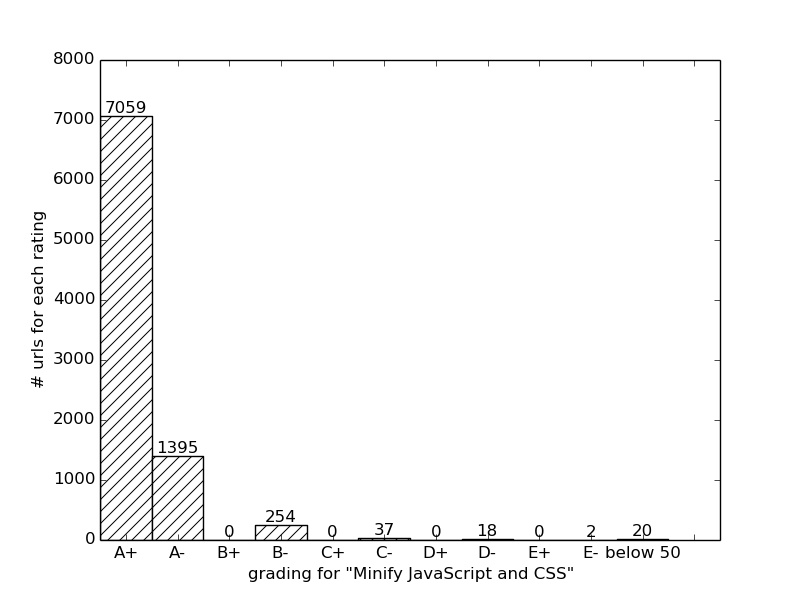
\includegraphics[scale=0.33]{new-img-jpg/deploy-jpg/Minify JavaScript and CSS.jpg}
        \caption{'Minify JavaScript and CSS' rule without PageSpeed }
        \label{fig:minify-nopagespeed}
    \end{subfigure}
    \caption{Comparing 'Minify JavaScript and CSS' rule}
    \label{fig:minify-comparison}
\end{figure*}
%\begin{center}
%\end{center}
\end{document}
